% Figure 2 — Fusion strategies compared (MoR Fig.2 레이아웃: (a)(b)(c) 세 패널).
%   (a) early fusion (concat): 세 브랜치 -> L2 -> concat 272 -> Cox head 하나, end-to-end
%   (b) late fusion, three-way: 세 축 각각 독립 학습 -> r_img, r_clin, r_rep -> CoxPH(3)
%   (c) late fusion, two-way (ours): tabular arm(임상+판독지 공동학습) + image arm -> CoxPH(2)
% 점선 상자 = 독립적으로 학습되는 모델 하나. 수치 출처: src/sclc/model.py, MODEL_SUMMARY.md §3.
\documentclass[tikz,border=6pt]{standalone}
% 논문 그림 공통 스타일 (fig1/fig2 가 \input 한다).
% 시각 언어는 Mixture-of-Recursions(MoR) 논문 Fig.1/2 를 따른다:
%   파스텔 채움 + 진남색 얇은 윤곽 + 둥근 모서리, 산세리프 라벨.
% 색 의미(두 그림에서 동일):
%   boxblue   = 영상 모달리티      boxpurple = 임상 모달리티     boxpink = 판독지 모달리티
%   boxgray   = 일반 연산 블록     boxyellow = Cox 관련(head/combiner)
%   dashed    = 동결(frozen) 사전학습 모듈
\usepackage[T1]{fontenc}
\usepackage{helvet}
\renewcommand{\familydefault}{\sfdefault}
\usepackage{amsmath,amssymb}
\usetikzlibrary{positioning,arrows.meta,calc,fit,backgrounds}

\definecolor{navy}{HTML}{2F3B52}
\definecolor{ink}{HTML}{1A1A1A}
\definecolor{ink2}{HTML}{5A5E66}
\definecolor{boxblue}{HTML}{CFE0F7}
\definecolor{boxpink}{HTML}{F6CDD0}
\definecolor{boxpurple}{HTML}{DCD6F3}
\definecolor{boxyellow}{HTML}{FDEEB8}
\definecolor{boxgray}{HTML}{E9E9E9}
\definecolor{cellhold}{HTML}{3F5A8A}
\definecolor{cellfit}{HTML}{F8DD8A}
\definecolor{celleval}{HTML}{F2A4A8}

\tikzset{
  every node/.style={text=ink},
  blk/.style={draw=navy, line width=0.7pt, rounded corners=2.5pt, fill=#1,
              inner xsep=4pt, inner ysep=3pt, font=\footnotesize, align=center},
  blk/.default=boxgray,
  lay/.style={blk=#1, minimum width=30mm, minimum height=6mm},
  inp/.style={blk=#1, minimum width=15mm, minimum height=7mm},
  frozen/.style={lay=boxgray, dashed},
  container/.style={draw=navy, line width=0.8pt, rounded corners=6pt, fill=white, inner sep=6pt},
  armbox/.style={draw=navy, line width=0.6pt, dashed, rounded corners=5pt, inner sep=4pt},
  arr/.style={-{Latex[length=2.2mm,width=1.7mm]}, draw=navy, line width=0.75pt},
  lab/.style={font=\scriptsize, text=ink2, align=center, inner sep=1pt},
  op/.style={circle, draw=navy, line width=0.7pt, fill=white, inner sep=0pt,
             minimum size=4.2mm, font=\scriptsize},
  risk/.style={font=\footnotesize, inner sep=2pt},
  stage/.style={font=\scriptsize\itshape, text=ink2, inner sep=1pt},
  ptitle/.style={font=\footnotesize, align=center, inner sep=2pt},
}

% ---------------------------------------------------------------------------
% 입력 모달리티 아이콘 (fig2 입력단). 글자 라벨 대신 실제 PET-CT MIP 한 장 +
% 임상 표 / 판독지 문서 픽토그램을 쓴다. 모두 약 10.5mm x 12mm 로 크기를 맞추고
% 채움색은 모달리티 색(boxblue/boxpurple/boxpink), 윤곽은 navy 로 본문 도형과 통일.
%   사용: \iconimage{노드이름}{(x,y)}  등. 노드이름으로 화살표를 걸 수 있다.
\newcommand{\iconimage}[2]{%
  \node[blk=boxblue, inner sep=1.1pt, minimum width=0pt, minimum height=0pt] (#1) at #2
       {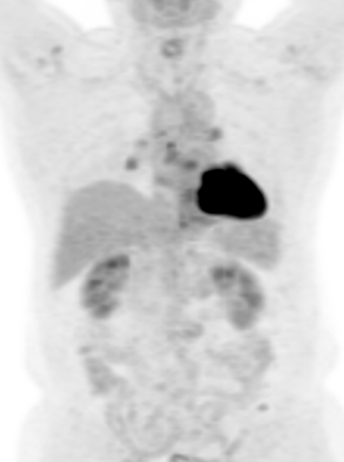
\includegraphics[height=11.8mm]{assets/pet_mip_icon.png}};%
}
\newcommand{\iconclinical}[2]{%
  \begin{scope}[shift={#2}]
    \begin{scope}
      \clip[rounded corners=2.5pt] (-5.25mm,-6mm) rectangle (5.25mm,6mm);
      \fill[boxpurple] (-5.25mm,-6mm) rectangle (5.25mm,6mm);
      \fill[navy!28]   (-5.25mm,3.3mm) rectangle (5.25mm,6mm);
      \draw[navy!45, line width=0.35pt]
        (-5.25mm,3.3mm) -- (5.25mm,3.3mm)  (-5.25mm,0.8mm) -- (5.25mm,0.8mm)
        (-5.25mm,-1.7mm) -- (5.25mm,-1.7mm) (-5.25mm,-4.2mm) -- (5.25mm,-4.2mm)
        (-1.75mm,-6mm) -- (-1.75mm,6mm)     (1.75mm,-6mm) -- (1.75mm,6mm);
    \end{scope}
    \draw[navy, line width=0.7pt, rounded corners=2.5pt] (-5.25mm,-6mm) rectangle (5.25mm,6mm);
    \node[minimum width=10.5mm, minimum height=12mm, inner sep=0pt] (#1) at (0,0) {};
  \end{scope}%
}
\newcommand{\iconreport}[2]{%
  \begin{scope}[shift={#2}]
    \fill[boxpink] (-4.6mm,-6mm) -- (-4.6mm,6mm) -- (1.7mm,6mm) -- (4.6mm,3.1mm) -- (4.6mm,-6mm) -- cycle;
    \draw[navy, line width=0.7pt, rounded corners=1pt]
      (-4.6mm,-6mm) -- (-4.6mm,6mm) -- (1.7mm,6mm) -- (4.6mm,3.1mm) -- (4.6mm,-6mm) -- cycle;
    \fill[navy!20] (1.7mm,6mm) -- (1.7mm,3.1mm) -- (4.6mm,3.1mm) -- cycle;
    \draw[navy, line width=0.55pt] (1.7mm,6mm) -- (1.7mm,3.1mm) -- (4.6mm,3.1mm);
    \draw[navy!55, line width=0.5pt]
      (-2.9mm,1.4mm) -- (2.9mm,1.4mm)  (-2.9mm,-0.4mm) -- (2.9mm,-0.4mm)
      (-2.9mm,-2.2mm) -- (2.9mm,-2.2mm) (-2.9mm,-4.0mm) -- (0.9mm,-4.0mm);
    \node[minimum width=9.2mm, minimum height=12mm, inner sep=0pt] (#1) at (0,0) {};
  \end{scope}%
}


% 세 패널이 공유하는 입력 + 모달리티 브랜치 (좌표는 scope 안에서 상대).
\newcommand{\inputsandbranches}{%
  % 입력단은 글자 대신 모달리티 아이콘: 실제 PET-CT MIP 한 장 / 임상 변수 표 / 판독지 문서.
  \iconimage{xi}{(0,-0.3)}
  \iconclinical{xc}{(1.9,-0.3)}
  \iconreport{xr}{(3.8,-0.3)}
  \node[lay=boxblue,   minimum width=16mm] (bi) at (0,1.15)   {CNN};
  \node[lay=boxpurple, minimum width=16mm] (bc) at (1.9,1.15) {MLP};
  \node[lay=boxpink,   minimum width=16mm, font=\scriptsize] (br) at (3.8,1.15) {RadBERT--MLP};
  \draw[arr] (xi) -- (bi); \draw[arr] (xc) -- (bc); \draw[arr] (xr) -- (br);
}

\begin{document}
\begin{tikzpicture}[x=1cm,y=1cm]

% ===================== (a) early fusion (concat) =====================
\begin{scope}[shift={(0,0)}]
  \inputsandbranches
  \node[op] (li) at (0,1.95)   {$\ell_2$};
  \node[op] (lc) at (1.9,1.95) {$\ell_2$};
  \node[op] (lr) at (3.8,1.95) {$\ell_2$};
  \node[blk, minimum width=52mm]           (cat) at (1.9,2.7)  {concat: $128\oplus128\oplus16=272$};
  \node[blk=boxyellow, minimum width=52mm] (hd)  at (1.9,3.45) {Cox head (one loss, one schedule)};
  \node[risk] (o) at (1.9,4.2) {risk};
  \draw[arr] (bi) -- (li); \draw[arr] (bc) -- (lc); \draw[arr] (br) -- (lr);
  \draw[arr] (li.north) -- (li.north |- cat.south);
  \draw[arr] (lc.north) -- (lc.north |- cat.south);
  \draw[arr] (lr.north) -- (lr.north |- cat.south);
  \draw[arr] (cat) -- (hd); \draw[arr] (hd) -- (o);
  \begin{scope}[on background layer]
    \node[armbox, fit=(bi)(br)(hd)] {};
  \end{scope}
  \node[ptitle] at (1.9,-1.35) {(a) Early fusion (concat)};
\end{scope}

% ===================== (b) late fusion, three-way =====================
\begin{scope}[shift={(6.5,0)}]
  \inputsandbranches
  \node[blk=boxyellow, minimum width=16mm] (hi) at (0,1.95)   {Cox head};
  \node[blk=boxyellow, minimum width=16mm] (hc) at (1.9,1.95) {Cox head};
  \node[blk=boxyellow, minimum width=16mm] (hr) at (3.8,1.95) {Cox head};
  \node[risk] (ri) at (0,2.7)   {$r_{\text{img}}$};
  \node[risk] (rc) at (1.9,2.7) {$r_{\text{clin}}$};
  \node[risk] (rr) at (3.8,2.7) {$r_{\text{rep}}$};
  \node[blk=boxyellow, minimum width=52mm, minimum height=9.5mm] (cb) at (1.9,3.6)
        {\textbf{Cox PH combiner}\\ $\beta_{\text{img}}r_{\text{img}}+\beta_{\text{clin}}r_{\text{clin}}+\beta_{\text{rep}}r_{\text{rep}}$};
  \node[risk] (o) at (1.9,4.5) {risk};
  \draw[arr] (bi) -- (hi); \draw[arr] (bc) -- (hc); \draw[arr] (br) -- (hr);
  \draw[arr] (hi) -- (ri); \draw[arr] (hc) -- (rc); \draw[arr] (hr) -- (rr);
  \draw[arr] (ri.north) -- (ri.north |- cb.south);
  \draw[arr] (rc.north) -- (rc.north |- cb.south);
  \draw[arr] (rr.north) -- (rr.north |- cb.south);
  \draw[arr] (cb) -- (o);
  \begin{scope}[on background layer]
    \node[armbox, fit=(bi)(hi)] {};
    \node[armbox, fit=(bc)(hc)] {};
    \node[armbox, fit=(br)(hr)] {};
  \end{scope}
  \node[ptitle] at (1.9,-1.35) {(b) Late fusion, three-way};
\end{scope}

% ===================== (c) late fusion, two-way (ours) =====================
\begin{scope}[shift={(13.0,0)}]
  \inputsandbranches
  % tabular arm: clinical + report trained jointly
  \node[op] (lc) at (1.9,1.95) {$\ell_2$};
  \node[op] (lr) at (3.8,1.95) {$\ell_2$};
  \node[blk, minimum width=33mm]           (cat) at (2.85,2.7)  {concat: $128\oplus16$};
  \node[blk=boxyellow, minimum width=33mm] (ht)  at (2.85,3.45) {Cox head};
  \node[risk] (rt) at (2.85,4.2) {$r_{\text{tab}}$};
  % image arm
  \node[blk=boxyellow, minimum width=16mm] (hi) at (0,3.45) {Cox head};
  \node[risk] (ri) at (0,4.2) {$r_{\text{img}}$};
  % combiner
  \node[blk=boxyellow, minimum width=54mm, minimum height=9.5mm] (cb) at (1.9,5.1)
        {\textbf{Cox PH combiner}\\ $\beta_{\text{tab}}r_{\text{tab}}+\beta_{\text{img}}r_{\text{img}}$};
  \node[risk] (o) at (1.9,6.0) {risk};
  \draw[arr] (bc) -- (lc); \draw[arr] (br) -- (lr);
  \draw[arr] (lc.north) -- (lc.north |- cat.south);
  \draw[arr] (lr.north) -- (lr.north |- cat.south);
  \draw[arr] (cat) -- (ht); \draw[arr] (ht) -- (rt);
  \draw[arr] (bi) -- (hi);  \draw[arr] (hi) -- (ri);
  \draw[arr] (ri.north) -- (ri.north |- cb.south);
  \draw[arr] (rt.north) -- (rt.north |- cb.south);
  \draw[arr] (cb) -- (o);
  \begin{scope}[on background layer]
    \node[armbox, fit=(bi)(hi)] (imarm) {};
    \node[armbox, fit=(bc)(br)(cat)(ht)] (tabarm) {};
  \end{scope}
  % arm 이름은 캡션에서 설명한다 (상자 위 라벨은 r_img/r_tab 화살표와 겹친다).
  \node[ptitle] at (1.9,-1.35) {(c) Late fusion, two-way (ours)};
\end{scope}

\end{tikzpicture}
\end{document}
